\documentclass[tikz]{standalone}
\usepackage{graphicx}
\usepackage[sfdefault]{universalis}
\usetikzlibrary{positioning}

\begin{document}
\small
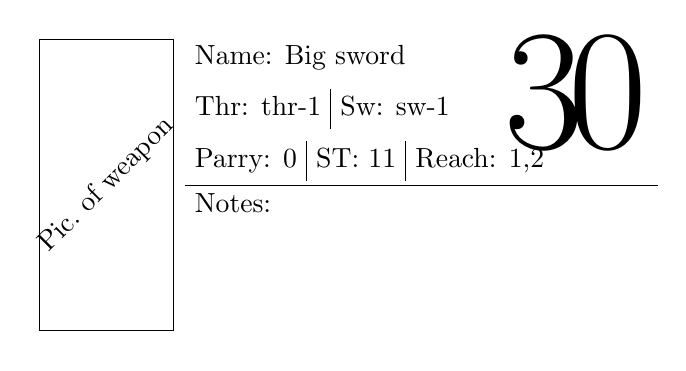
\begin{tikzpicture}
  \def\ro{0.15}
  \def\xlineskip{0.66cm}
  \def\xsep{\rule[-.4\baselineskip]{0.3pt}{1.2\baselineskip}}
  \def\xstrut{\rule[-.4\baselineskip]{0pt}{1.2\baselineskip}}
  % \draw [use as bounding box] (0,0) -- (1,1);
  % \draw (-1, -1) -- (0, 1);
  \coordinate (topcorner) at (8,4);
  \coordinate (picture top right) at (2,4);

  \draw[use as bounding box, draw=none] (0, 0) -- (topcorner);
  \draw ({0+\ro},{0+\ro}) rectangle ({2-\ro}, {4-\ro}) node[pos=.5, rotate=45] {Pic.~of weapon};
  \draw (2, 2) -- (8, 2);
  % Points cost
  \node [below left = 0.0cm and 0.0cm of topcorner, anchor=north east] (points cost) {\scalebox{2.5}{\Huge 3\hspace{-0.2ex}0}};
  % Name
  \node [right = 0pt of picture top right, anchor=north west] (name) {\xstrut Name: Big sword};
  % Damage (thrust)
  \node [below = \xlineskip of picture top right, anchor=north west] (thrust) {\strut %
    Thr: thr-1~\xsep~Sw: sw-1};
  % \node [below = 0pt of name] {Thrust: thr-1};
  % Damage (swing)
  % \node [right = 0.03cm of thrust] (swing) {\strut Sw: sw-1};
  % \node [below = 0pt of name] {TL: 10};
  % Reach
  % Parry
  \node [below = {2*\xlineskip} of picture top right, anchor=north west] (parry) {\strut %
    Parry: 0~\xsep~ST: 11~\xsep~Reach: 1,2};
  \node [below = {3*\xlineskip} of picture top right, anchor=north west] {Notes:};
  % ST
  % \node [right = 0.1cm of parry] (st) {\strut ST: 11};
  % Cost?
  % Weight
  % TL
  % \node [below = {3*\xlineskip} of picture top right, anchor=north west] (TL) {\strut TL: 10};
  % Notes
\end{tikzpicture}
\end{document}

%%% Local Variables:
%%% mode: latex
%%% TeX-master: "main"
%%% End:
